\documentclass[a4paper, 11pt]{article}
\usepackage{amsmath}
\usepackage{graphicx}
\usepackage{geometry}
\usepackage{listings}
\geometry{scale=0.8}
\linespread{1.5}
\usepackage{hyperref}
\usepackage{xcolor}
\usepackage[UTF8, scheme = plain]{ctex}
\usepackage{float}
\usepackage{listings}
\usepackage{enumitem}


\title{	
\normalfont \normalsize
\textsc{School of Data and Computer Science, Sun Yat-sen University} \\ [25pt] %textsc small capital letters
\rule{\textwidth}{0.5pt} \\[0.4cm] % Thin top horizontal rule
\huge  P03 Planning and Uncertainty\\ % The assignment title
\rule{\textwidth}{2pt} \\[0.5cm] % Thick bottom horizontal rule
\author{}
\date{Due: 11:59pm, Saturday, Nov. 28, 2020}
}

\begin{document}
\maketitle
\tableofcontents
\newpage
\section{STRIPS planner}
In this part, you will implement a simple STRIPS planner. The input of your planner is a PDDL domain file and a problem file in the STRIPS restriction, that is, preconditions of actions and the goal are conjunctions of atoms, and effects of actions are conjunctions of literals. The output of your planner is a sequence of actions to achieve the goal.

\begin{enumerate}

\item Describe with sentences the main ideas behind computing the heuristic for a state using reachability analysis from lecture notes. (10 points)
\textbf{解答:}
	\textbf{搜索问题}
    首先,在STRIPS规划中,我们把Planning看作一种搜索问题,状态表示为封闭世界知识库,初始的知识库是初始状态,动作则认为是把一个状态映射到另一个状态上,由于封闭世界假设,我们很容易验证目标是否在目前的知识库中,也就是是否已经达成。
    \textbf{松弛问题}
    但是问题在于当搜索树过大的时候会需要利用松弛问题的启发值,用启发式算法来确定下一个搜索的节点,才会比较快速找到我们的目标解,接下来我们阐述用可达性分析来获得启发式函数值的思想:
    
    当每个动作的前提都是正向的事实(不是Not),并且目标也是正向事实,把原问题放松为动作的效果,只考虑add列表,而不考虑delete列表对问题的知识库的影响,则这样动作的前提更容易被满足,因此很多之前问题不可做的问题也可以做了。有定理指出:松弛问题的解的长度小于等于原问题的解的长度,因此是可采纳的。
    \textbf{可达性分析}
    计算启发式值的时候,我们用逐步建立状层态S和动作层A的方法,来获得我们在此松弛问题下,需要多少步动作能够到达目标,作为启发式值。
    
    首先开始于初始状态$S_0$,接下来找所有前提已经在$S_0$中的动作,组成$A_0$,下一层的$S_1$是$S_0$并上$A_0$的add效果列表,之后继续这个过程。其中$A_i$表示前提在$S_i$中,但是动作没有出现在上一个动作层$A_{i-1}$的动作,而状态层$S_i$是上一个动作层和本次能新进行的动作添加列表的并集。
    
    最后直到目标全部含于当前状态层,或者状态层不再改变,则终止算法。如果这个时候状态层没有目标,则不可达;反之,就可达,并且此时的动作数就是启发式函数值。
    
    动作数的计算方法如下:首先找出能够涵盖目标状态的最小动作集A,把当前状态层划分为该动作集的添加效果$G_N$其他部分为第二部分,$G_P$,后者和A的前提集合的并集作为下一回的调用参数,接下来继续在size(A)的基础上加上递归调用此函数在上一层的动作数。
    
    

\item Implement a STRIPS planner by using A$^*$ search and the heuristic function you implemented.(20 points)
\textbf{思路}
	我们为了代码的整洁性,在数据结构方面,用一个大类Problem来涵盖整个搜索问题的相关函数及变量,包括当前的状态,目标状态,以及动作列表等。并把搜索函数,寻找可用的动作等函数定义在里面。Action类作为一个内部类定义在Problem中,含有前提,添加,删除等列表及其他变量,以及判断此动作当前是否可做,更新状态,回溯状态等操作。
	
	这里我们的逻辑是这样的,首先由main调用函数,获取初始状态可做的动作,然后进入solve函数,寻找可做的动作,并用启发式值和cost排序为优先级队列,取队首动作执行,并更新状态,递归继续搜索过程,若判断可做动作为空,则回退一个动作。
	
	\textbf{递归搜索函数}
	\begin{lstlisting}
    def solve(self, actions):
        # 获取第一个动作
        theAction = actions.get()[1]
        aaaaaction = [theAction.name]
        for val in theAction.instance.values():
            aaaaaction.append(val)
        # print(aaaaaction)
        # 做这个动作
        theAction.do()
        self.cost += 1
        Problem.solves.append(theAction)
        is_goal = True
        for goal in Problem.goalState:
            if goal not in Problem.nowState:
                is_goal = False
        if is_goal:
            return True
        # if Problem.goalState in Problem.nowState:
        #     return True

        actionsb = self.changeActionstoQueue()
        if actionsb:
            return self.solve(actionsb)
        # 如果运行到这了就说明这个动作会导致问题无解,回溯
        theAction.pullBack()
        self.cost -= 1
        Problem.solves.remove(theAction)	
	\end{lstlisting}
\item Explain any ideas you use to speed up the implementation. (10 points)
	在判断动作是否可做的时候,我们没有去遍历动作含有的变量的类型,再遍历该类型所有实例化,来构造实例化新的Action对象,再去判断前提是否涵盖于当前状态。
	
	而是选择去遍历所有Problem文件出现的所有实例化的变量,不管类型,做一个排列,之后对每个排列来判断类型和动作变量表是否相匹配。原因在于我们的问题中,实例化的变量个数还算较少,遍历他们的排列比起遍历类型来说更迅速。
	
	如[move,p,l1,l2],(p-player,l1-location,l2-location),读文件之后,player只有npc一个,location有town,field,castle三个,不去根据player、location去找对应的npc,town,field,castle,而是通过如[npc,town,field]这样的排列判断是否符合类型。
	
	还有在于对前提是否在状态的判断,我们并非全部实例化完动作的pre,add,del之后再判断,而是对前提的每一项,挨个实例化,判断是否存在,一旦有一个不存在,就判断出不可做。不再继续,break出来,减少不必要的实例化。
\item Run you planner on the 5 test cases, and report the returned plans and the running times. Analyse the experimental results. (10 points)
	\textbf{test case 0}
	\begin{figure}[H]
	\centering
	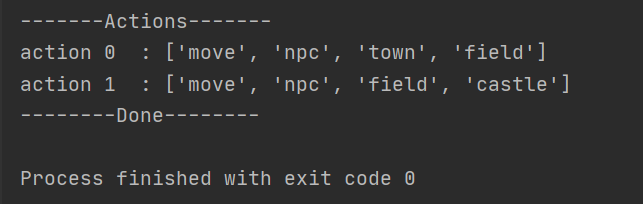
\includegraphics[width=1\textwidth]{Pic/test0.png}
	\caption{test0 result}
	\end{figure}
	
	\textbf{test case 1}
	\begin{figure}[H]
	\centering
	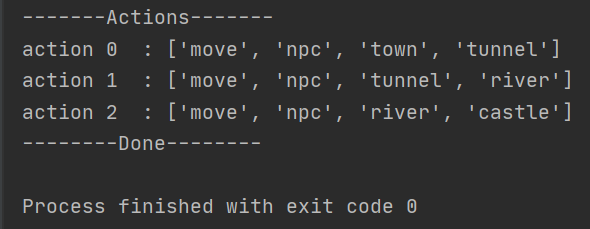
\includegraphics[width=1\textwidth]{Pic/test1.png}
	\caption{test2 result}
	\end{figure}
	
%	\textbf{test case 2}
%	\begin{figure}[H]
%	\centering
%	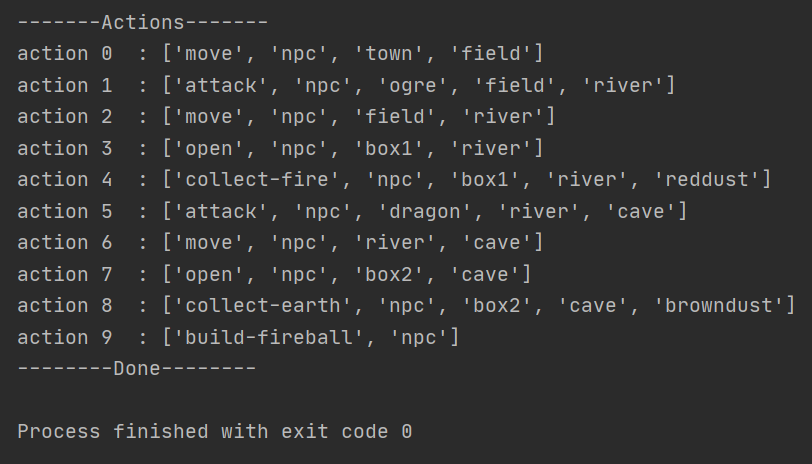
\includegraphics[width=1\textwidth]{Pic/test2.png}
%	\caption{test2 result}
%	\end{figure}
	
	\textbf{test case 3}
	\begin{figure}[H]
	\centering
	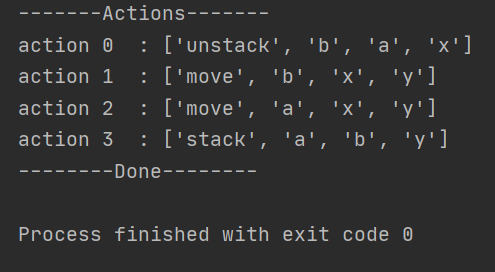
\includegraphics[width=1\textwidth]{Pic/test3.png}
	\caption{test3 result}
	\end{figure}
	
	\textbf{test case 4}
	\begin{figure}[H]
	\centering
	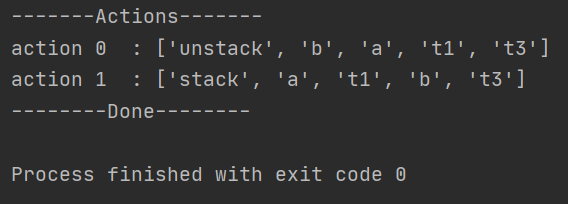
\includegraphics[width=1\textwidth]{Pic/test4.png}
	\caption{test4 result}
	\end{figure}
		
\end{enumerate}


\section{Diagnosing by Bayesian Networks}
\textbf{2.1 Variables and their domais}
\begin{lstlisting}{language=Python}
(1)PatientAge:['0-30','31-65','65+']
(2)CTScanResult:['Ischemic Stroke','Hemmorraghic Stroke']
(3)MRIScanResult: ['Ischemic Stroke','Hemmorraghic Stroke']
(4)StrokeType: ['Ischemic Stroke','Hemmorraghic Stroke', 'Stroke Mimic']
(5)Anticoagulants: ['Used','Not used']
(6)Mortality:['True', 'False']
(7)Disability: ['Negligible', 'Moderate', 'Severe']
\end{lstlisting}
\textbf{2.2 CPTs}

\textbf{Note:} [CTScanResult, MRIScanResult,StrokeType] means:

P(StrokeType='...' $|$ CTScanResult='...' $\land$  MRIScanResult='...')
\begin{lstlisting}{language=Python}
(1)
[PatientAge]

['0-30', 0.10],
['31-65', 0.30],
['65+', 0.60]

(2)
[CTScanResult]

['Ischemic Stroke',0.7],
[ 'Hemmorraghic Stroke',0.3]

(3)
[MRIScanResult]

['Ischemic Stroke',0.7],
[ 'Hemmorraghic Stroke',0.3]

(4)
[Anticoagulants]

[Used',0.5],
['Not used',0.5]

(5)
[CTScanResult, MRIScanResult,StrokeType])

['Ischemic Stroke','Ischemic Stroke','Ischemic Stroke',0.8],
['Ischemic Stroke','Hemmorraghic Stroke','Ischemic Stroke',0.5],
[ 'Hemmorraghic Stroke','Ischemic Stroke','Ischemic Stroke',0.5],
[ 'Hemmorraghic Stroke','Hemmorraghic Stroke','Ischemic Stroke',0],

['Ischemic Stroke','Ischemic Stroke','Hemmorraghic Stroke',0],
['Ischemic Stroke','Hemmorraghic Stroke','Hemmorraghic Stroke',0.4],
[ 'Hemmorraghic Stroke','Ischemic Stroke','Hemmorraghic Stroke',0.4],
[ 'Hemmorraghic Stroke','Hemmorraghic Stroke','Hemmorraghic Stroke',0.9],

['Ischemic Stroke','Ischemic Stroke','Stroke Mimic',0.2],
['Ischemic Stroke','Hemmorraghic Stroke','Stroke Mimic',0.1],
[ 'Hemmorraghic Stroke','Ischemic Stroke','Stroke Mimic',0.1],
[ 'Hemmorraghic Stroke','Hemmorraghic Stroke','Stroke Mimic',0.1],

(6)
[StrokeType, Anticoagulants, Mortality]

['Ischemic Stroke', 'Used', 'False',0.28],
['Hemmorraghic Stroke', 'Used', 'False',0.99],
['Stroke Mimic', 'Used', 'False',0.1],
['Ischemic Stroke','Not used', 'False',0.56],
['Hemmorraghic Stroke', 'Not used', 'False',0.58],
['Stroke Mimic', 'Not used', 'False',0.05],

['Ischemic Stroke',  'Used' ,'True',0.72],
['Hemmorraghic Stroke', 'Used', 'True',0.01],
['Stroke Mimic', 'Used', 'True',0.9],
['Ischemic Stroke',  'Not used' ,'True',0.44],
['Hemmorraghic Stroke', 'Not used', 'True',0.42 ],
['Stroke Mimic', 'Not used', 'True',0.95]

(7)
[StrokeType, PatientAge, Disability]

['Ischemic Stroke',   '0-30','Negligible', 0.80],
['Hemmorraghic Stroke', '0-30','Negligible', 0.70],
['Stroke Mimic',        '0-30', 'Negligible',0.9],
['Ischemic Stroke',     '31-65','Negligible', 0.60],
['Hemmorraghic Stroke', '31-65','Negligible', 0.50],
['Stroke Mimic',        '31-65', 'Negligible',0.4],
['Ischemic Stroke',     '65+'  , 'Negligible',0.30],
['Hemmorraghic Stroke', '65+'  , 'Negligible',0.20],
['Stroke Mimic',        '65+'  , 'Negligible',0.1],

['Ischemic Stroke',     '0-30' ,'Moderate',0.1],
['Hemmorraghic Stroke', '0-30' ,'Moderate',0.2],
['Stroke Mimic',        '0-30' ,'Moderate',0.05],
['Ischemic Stroke',     '31-65','Moderate',0.3],
['Hemmorraghic Stroke', '31-65','Moderate',0.4],
['Stroke Mimic',        '31-65','Moderate',0.3],
['Ischemic Stroke',     '65+'  ,'Moderate',0.4],
['Hemmorraghic Stroke', '65+'  ,'Moderate',0.2],
['Stroke Mimic',        '65+'  ,'Moderate',0.1],

['Ischemic Stroke',     '0-30' ,'Severe',0.1],
['Hemmorraghic Stroke', '0-30' ,'Severe',0.1],
['Stroke Mimic',        '0-30' ,'Severe',0.05],
['Ischemic Stroke',     '31-65','Severe',0.1],
['Hemmorraghic Stroke', '31-65','Severe',0.1],
['Stroke Mimic',        '31-65','Severe',0.3],
['Ischemic Stroke',     '65+'  ,'Severe',0.3],
['Hemmorraghic Stroke', '65+'  ,'Severe',0.6],
['Stroke Mimic',        '65+'  ,'Severe',0.8]
\end{lstlisting}

\textbf{2.3 Tasks}

\begin{enumerate}
\item Briefly describe with sentences the main ideas of  the VE algorithm. (10 points)
\paragraph{VE algorithm}
在计算给定证据下某些变量的结果的时候,我们要应用链式法则和全概公式来计算,其中链式法则将表达式拆解成乘积的形式,而全概公式将表达式拆解成求合的形式。再通过限制住某些元素得到取值来得到我们最终想要的结果。VE算法通过restrict(限制变量的取值),multiply(进行链式法则实现概率之间的相乘),sumout(全概公式求合)三个操作,将无关变量通过相乘求合等操作消去,留下在证据下我们需要查询的变量的概率。

\item Implement the VE algorithm (C++ or Python) to calculate the following probability values: (10 points)
    
\begin{enumerate}
\item p1 = P(Mortality='True' $\land$ CTScanResult='Ischemic Stroke' $|$ PatientAge='31-65' )

\item p2 = P(Disability='Moderate' $\land$ CTScanResult='Hemmorraghic Stroke' $|$ PatientAge='65+' $\land$  MRIScanResult='Hemmorraghic Stroke')

\item p3 = P(StrokeType='Hemmorraghic Stroke' $|$ PatientAge='65+' $\land$ CTScanResult='Hemmorraghic Stroke' $\land$ MRIScanResult='Ischemic Stroke')

\item p4 = P(Anticoagulants='Used' $|$ PatientAge='31-65')

\item p5 = P(Disability='Negligible')
\end{enumerate}

\paragraph{实现思路}
有了实验八的基础,这一部分的代码只需要在实验八的基础上稍作修改即可。首先我们添加了一个名为valueMap的字典,里面讲每一个变量的可取值映射为0,1,2……这样做可以方便后续的数值选取。其次我们将原本传入的列表类型queryVariables换成了字典类型变量,并在其中记录每一个查询变量的查询取值,这样在输出结果的时候,只需要输出查询的取值结果而不需要输出全部的结果,相应地在printInf函数中做出一些格式化的调整。下面我们分别给出我们的程序计算的概率结果数值和使用pomegranate进行计算得到的结果,经过比对可以发现二者在误差可允许的范围内结果一致。会出现微小的误差是由变量消除的顺序导致的,因为消除的顺序不同所以计算的结果运算的顺序也不同。

\begin{figure}[H]
\centering
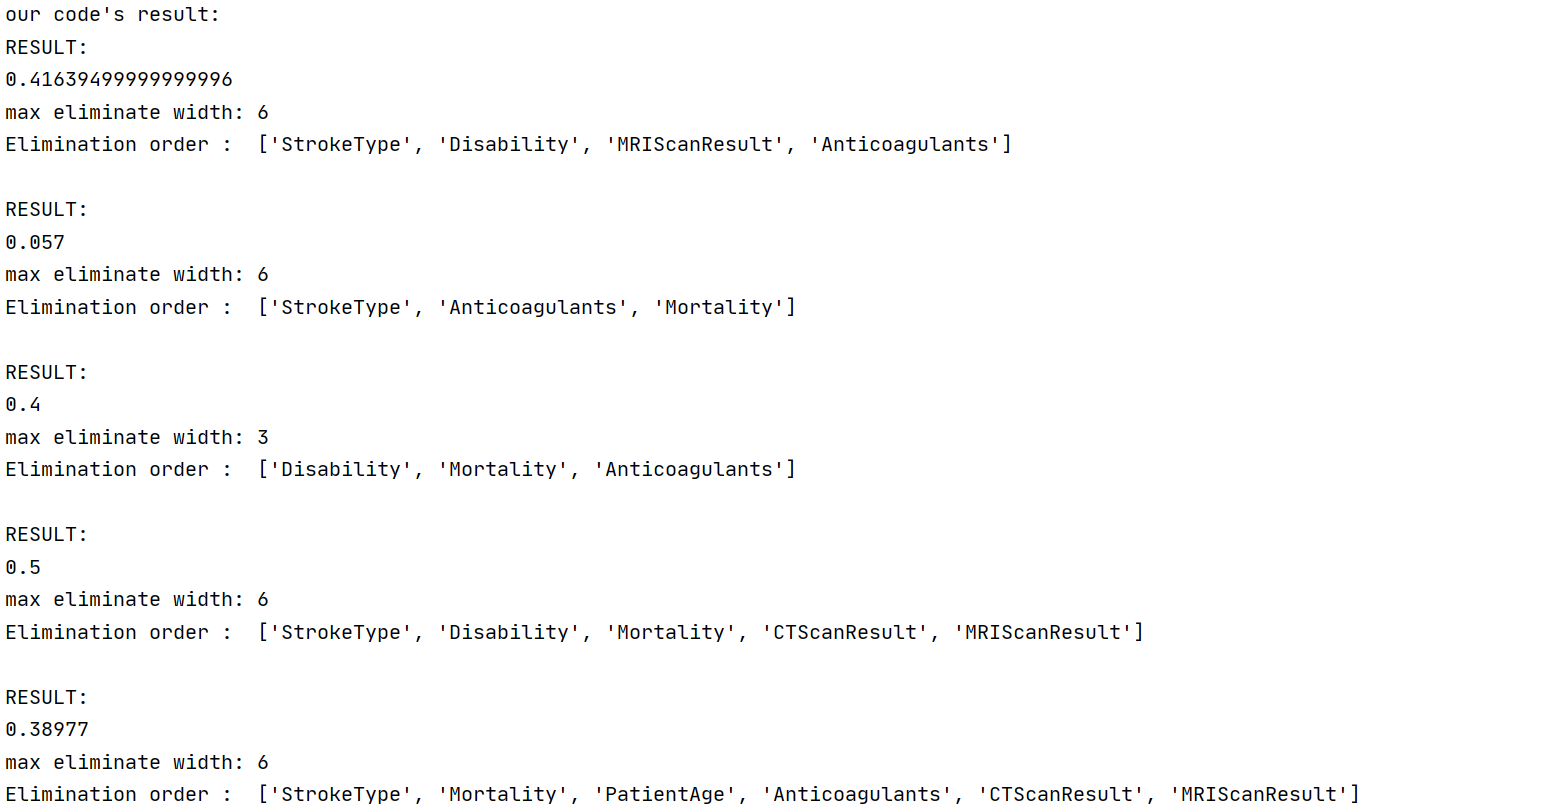
\includegraphics[width=1\textwidth]{Pic/un1.png}
\caption{our code's result}
\end{figure}

\begin{figure}[H]
\centering
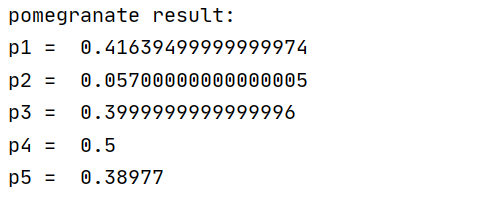
\includegraphics[width=0.5\textwidth]{Pic/un2.png}
\caption{pomegranate result}
\end{figure}

\item Implement an algorithm to select a good order of variable elimination. (10 points)
\paragraph{PolyTree}
根据给出的概率表,我们可以知道我们的这个问题是一个多叉树,变量之间的相互作用关系如下所示。对于贝叶斯网络中的多叉树来说,在每一步我们都消掉一个单一连接的节点(因为是多叉树,所以一定能保证在每一步消去的时候都有单一连接的节点),那么树的因子的大小将一直不会增加,也就是说,初始时因子中变量数目最大的一个即为树的宽度。
\begin{figure}[H]
\centering
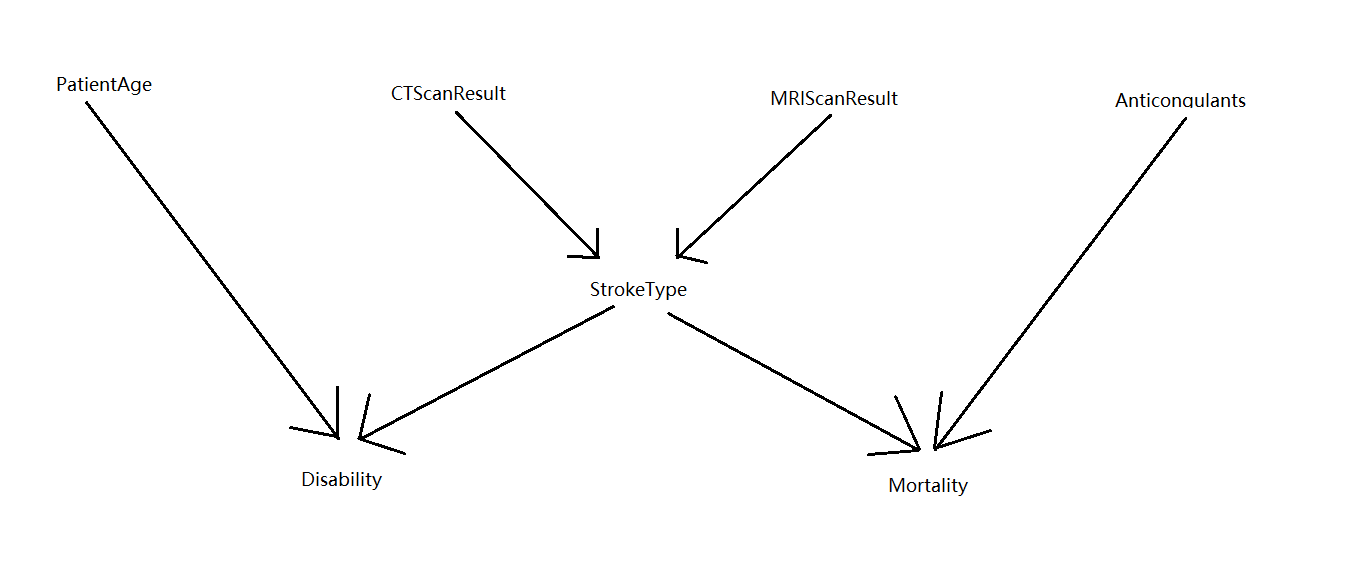
\includegraphics[width=1\textwidth]{Pic/un3.png}
\caption{the polytree of the problem}
\end{figure}
\paragraph{Min-Fill Heuristic}
我们使用的启发式策略是每次都消除产生最小因子的变量。这一算法在多树问题上是线性时间复杂度的。在多数问题中我们只需要在待消除变量中寻找单一连接的节点,然后在单一连接的节点中因子大小最小的变量先进行消除即可。这体现在我们的数据结构中只需要根据变量表的大小就可以判断。我们利用一个优先队列来帮助简化编程,具体代码如下所示。
\newline
\lstset{
    %backgroundcolor=\color{red!50!green!50!blue!50},%代码块背景色为浅灰色
    language=Python,
    rulesepcolor= \color{gray}, %代码块边框颜色
    breaklines=true,  %代码过长则换行
    numbers=left, %行号在左侧显示
    numberstyle= \small,%行号字体
    keywordstyle= \color{blue},%关键字颜色
    commentstyle=\color{gray}, %注释颜色
    frame=shadowbox%用方框框住代码块
    }
\begin{lstlisting}
def orderedVariables(factorList, orderedListOfHiddenVariables: list):
    q = queue.PriorityQueue()
    for v in orderedListOfHiddenVariables:
        for f in factorList:
            if v == f.name:
                q.put((len(f.varList), v))
                break
    orderedListOfHiddenVariables.clear()
    while q.qsize():
        orderedListOfHiddenVariables.append(q.get()[1])

\end{lstlisting}

\item Compare the running times of the VE algorithm for different orders of variable elimination, and fill out the following table: For test cases p4 and p5, for each of the order selected by your algorithm and 5 other orders, report the elimination with, and the total running time of the VE algorithm. For each case, the first order of elimination should be the one chosen by your algorithm. Analyze the results. (20 points)
\paragraph{} 由于问题模型很简单,即使是使用最差的消除顺序运行时间也很短,为了使结果更加明显,我们将每个消除顺序都运行5000次后比对运行时间的差异。在测试时,注释掉程序的输出部分,将待消除变量保存到一个列表中,之后调用我们实现的orderedVariables函数寻找最优消除顺序,之后调用random.shuffle(eliminatelist)函数来对消除顺序进行随机重排后进行消除宽度和时间上的测试。

\newcommand{\tabincell}[2]{\begin{tabular}{@{}#1@{}}#2\end{tabular}} 
\begin{tabular}{|c|c|c|c|}
\hline
Test case                                                                                             & Elimination order & Elimination width  & Total time \\ \hline
p4  & 3 & \tabincell{c}{['CTScanResult', 'MRIScanResult',\\ 'Disability', 'Mortality', 'StrokeType'] } &  1.23 s          \\ \hline
p4  & 4 & \tabincell{c}{['MRIScanResult', 'Mortality', \\'StrokeType', 'Disability', 'CTScanResult'] } &  2.51 s          \\ \hline
p4  & 4 & \tabincell{c}{['CTScanResult', 'MRIScanResult',\\ 'StrokeType', 'Disability', 'Mortality'] } &  2.84 s          \\ \hline
p4  & 6 & \tabincell{c}{['StrokeType', 'Mortality', \\'MRIScanResult', 'CTScanResult', 'Disability'] } &  7.70 s          \\ \hline
p4  & 5 & \tabincell{c}{['CTScanResult', 'StrokeType', \\'MRIScanResult', 'Disability', 'Mortality'] } &  4.74 s          \\ \hline
p4  & 6 & \tabincell{c}{['StrokeType', 'Mortality', 'Disability',\\ 'CTScanResult', 'MRIScanResult'] } &  7.53 s          \\ \hline
p5  & 3 & \tabincell{c}{['Anticoagulants', 'CTScanResult', 'MRIScanResult',\\ 'PatientAge', 'Mortality', 'StrokeType']}    &   2.10 s    \\ \hline
p5  & 4 & \tabincell{c}{['MRIScanResult', 'PatientAge', 'StrokeType', \\'Anticoagulants', 'Mortality', 'CTScanResult']}    &   4.94 s    \\ \hline
p5  & 5 & \tabincell{c}{['CTScanResult', 'StrokeType', 'PatientAge', \\'Anticoagulants', 'Mortality', 'MRIScanResult']}    &   12.89 s   \\ \hline
p5  & 6 & \tabincell{c}{['StrokeType', 'Mortality', 'MRIScanResult',\\ 'Anticoagulants', 'PatientAge', 'CTScanResult']}    &   20.77s    \\ \hline
p5  & 4 & \tabincell{c}{['Anticoagulants', 'PatientAge', 'StrokeType',\\ 'MRIScanResult', 'Mortality', 'CTScanResult']}    &   4.40 s    \\ \hline
p5  & 6 & \tabincell{c}{['StrokeType', 'Anticoagulants', 'PatientAge',\\ 'Mortality', 'CTScanResult', 'MRIScanResult']}    &   22.61 s   \\ \hline
\end{tabular} 

\paragraph{结果截图展示}
\begin{figure}[H]
\centering
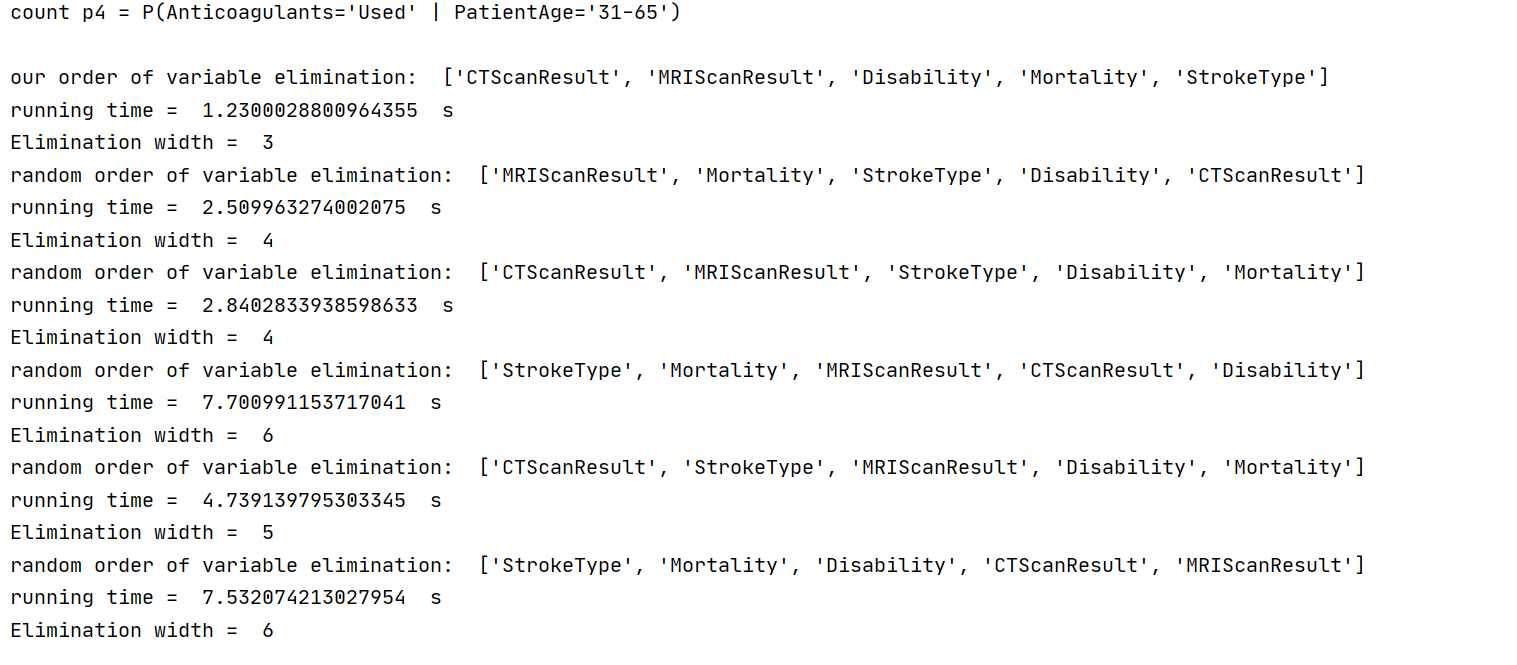
\includegraphics[width=1\textwidth]{Pic/un4.png}
\caption{p4 result}
\end{figure}
\begin{figure}[H]
\centering
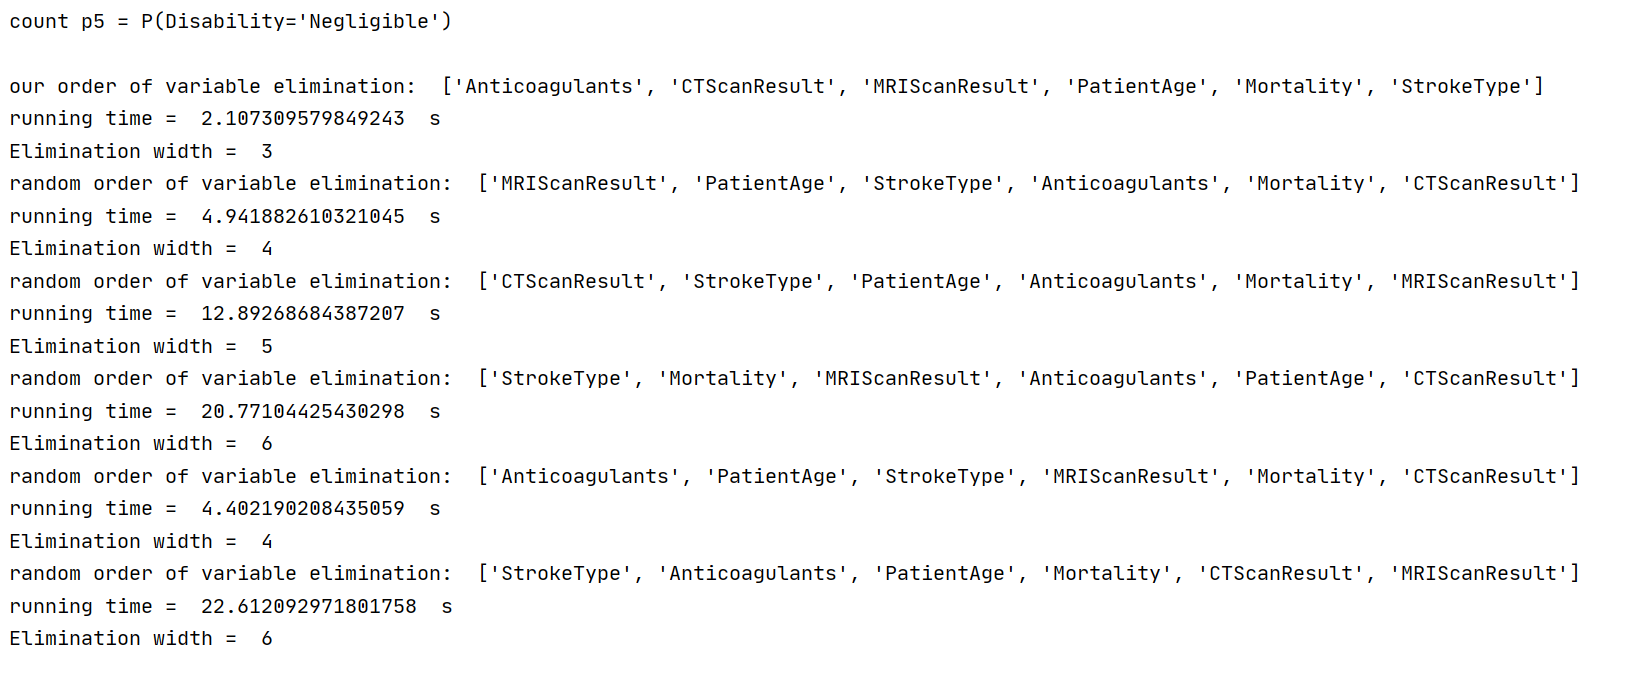
\includegraphics[width=1\textwidth]{Pic/un5.png}
\caption{p5 result}
\end{figure}
\paragraph{结果分析}
可以看出不同的变量消除顺序对于结果的影响是巨大的,而我们的算法找出的消除顺序无论是在消除宽度上还是运行时间上都有很好的效果。
\section{Due: 11:59pm, Saturday, Nov. 28, 2020}

 Please hand in a file named \textsf{P03\_YourNumber.pdf}, and send it to \textsf{ai\_2020@foxmail.com}
\end{enumerate}
\end{document}

\section{Due: 11:59pm, Saturday, Nov. 28, 2020}
